\documentclass[11pt]{article}
\usepackage{acl}
\usepackage{times}
\usepackage{latexsym}
\usepackage[T1]{fontenc}
\usepackage[utf8]{inputenc}
\usepackage{microtype}
\usepackage{graphicx}
\graphicspath{{../src/outputs/}}
\usepackage{booktabs}
\usepackage{amsmath}

\title{Group 29 Progress Report:\\
Early Prediction of Student Dropout and Academic Success}

\author{Anam Khan \and Haniya Kashif \\
  \texttt{\{khana489,kashih2\}@mcmaster.ca}}

\begin{document}
\maketitle

%% ---------------------------------------------------------------- 1
\section{Introduction}
Universities usually learn that a student is struggling only after the student has withdrawn or failed enough courses that recovery is unrealistic. Dropout is costly for students (debt without a degree), for institutions (lost tuition and weaker graduation statistics) and for society (a lower return on public education spending). Advisors cannot manually monitor thousands of students, so an automated early-warning system could let staff offer tutoring, financial aid or counselling while it still matters.
 
We build such a system as a three-class classifier (Dropout, Enrolled, Graduate) on tabular student records. Our central question is \emph{how early} a student's outcome can be predicted reliably. We ask the same question at three points in time with progressively more information: at enrollment (Stage~1), after semester~1 (Stage~2) and after semester~2 (Stage~3). A moderately accurate Stage~1 model may be more useful than a more accurate Stage~3 model, because only an early prediction leaves time to help. Anticipated challenges are class imbalance, the ambiguity of the ``Enrolled'' label, weak early signal, feature leakage across stages, and fairness.
 
This report describes our preliminary implementation: the dataset and preprocessing, leakage-safe stage-wise feature sets, a majority-class baseline, and three learned models (logistic regression, random forest and gradient boosting) evaluated at all three stages. Even at this early point, all learned models clearly beat the majority baseline (0.22 macro F1). Test macro F1 rises from about 0.52 at Stage~1 to about 0.71 at Stage~3, with most of the gain arriving once semester-1 information is available.
%% ---------------------------------------------------------------- 2
\section{Related Work}
\paragraph{Student retention and dropout prediction} Student retention has long been studied in education research; \citet{tinto1975} gave an influential theoretical account of dropout from higher education based on academic and social integration. More recent work applies machine learning to institutional records. Our dataset was created at a Portuguese polytechnic institute to support early identification of students at risk and was introduced by \citet{martins2021}, who used only information known at enrollment, tested synthetic oversampling to handle class imbalance, and compared standard classifiers with boosting algorithms, finding that boosting worked better; they listed first-year academic performance as future work. The same group later studied prediction at several phases of the enrollment year and found that random forests, combined with imbalance-handling strategies, performed best \citep{martins2023}. \citet{realinho2022} document the dataset itself: it merges several disjoint institutional databases and labels each student as Dropout, Enrolled or Graduate at the end of the normal course duration. Our work is closest to these phased studies, but differs in assigning each variable to a stage conservatively to avoid leakage (for example, placing payment status after enrollment), excluding Nationality from the main feature set, and planning explicit fairness, proxy-feature and calibration analyses across stages.
These papers motivate the task and provide the data. Our project differs in that we explicitly build one feature set per prediction point, assigning variables conservatively to avoid leakage, and compare models across those stages rather than treating all features as available at once.
 
\paragraph{Models for tabular data} For tabular data with mixed numeric and categorical features, tree ensembles are strong default choices. Random forests \citep{breiman2001} average many decorrelated trees, and gradient boosting \citep{friedman2001} builds trees sequentially to correct earlier errors. Efficient implementations such as XGBoost \citep{chen2016xgboost} and LightGBM \citep{ke2017lightgbm} are widely used; the histogram-based boosting in scikit-learn that we use follows the LightGBM design. \citet{grinsztajn2022} found that tree-based models often remain ahead of deep learning on medium-sized tabular datasets, which is why we focus on tree ensembles and use logistic regression as an interpretable baseline.
 
\paragraph{Imbalance, calibration and fairness} Because our classes are imbalanced, we also draw on work on imbalance and probability quality. \citet{chawla2002} proposed SMOTE oversampling, which we plan to compare against class weighting. \citet{niculescu2005} showed that predicted probabilities from many classifiers are poorly calibrated, motivating our planned calibration checks. For fairness, \citet{hardt2016} define group-level error criteria such as equality of opportunity, which we will use to compare error rates across groups (also why we exclude using nationality for now), and \citet{lundberg2017} provide SHAP, one option for interpreting predictions.
%% ---------------------------------------------------------------- 3
\section{Dataset}
We use the public UCI ``Predict Students' Dropout and Academic Success'' dataset (CC BY 4.0), which contains 4,424 student records with 36 features and one target label (Dropout, Enrolled or Graduate) drawn from the institution's records, so no manual annotation was needed. Features cover demographics, application and enrollment information, previous education, parents' education and occupation, scholarship and payment status, first- and second-semester curricular unit statistics, and three macroeconomic indicators (unemployment, inflation, GDP). The data are included with our submission (\texttt{data.csv}).

\paragraph{Class distribution} The classes are imbalanced: Graduate is 49.9\% of students (2,209), Dropout 32.1\% (1,421) and Enrolled 17.9\% (794) (Figure~\ref{fig:classes}). A majority-class predictor therefore reaches about 50\% accuracy but only 0.222 macro F1.

\begin{figure}[t]
  \centering
  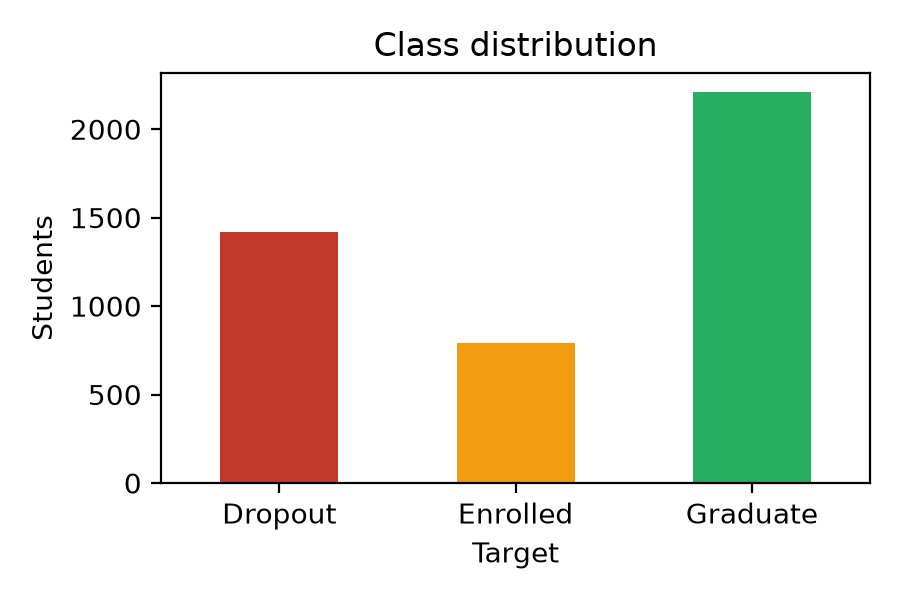
\includegraphics[width=0.7\columnwidth]{class_distribution.png}
  \caption{Class distribution of the 4,424 students.}
  \label{fig:classes}
\end{figure}

\paragraph{Preprocessing} The dataset documentation reports that anomalies and missing values were handled by its creators; we verified that there are no missing values and checked for duplicate rows. We stripped stray whitespace from column names, mapped the target to integers (Dropout=0, Enrolled=1, Graduate=2), and dropped the Nationality column from the main feature set because of fairness concerns. Eight nominal code columns (marital status, application mode, course, previous qualification, and the mothers' and fathers' qualification and occupation) are treated as categorical, since their integer codes carry no numeric meaning. All other columns are used as numeric or binary values.

\paragraph{Split} We make one stratified 80/20 split (3,539 training and 885 test students) with a fixed random seed. The same split is reused for every stage and model so that stage comparisons are fair. The test set is used only to report final numbers.

%% ---------------------------------------------------------------- 4
\section{Features}
\paragraph{Stage-wise feature sets} We assign each variable to the earliest stage at which it would be known (Table~\ref{tab:stages}). Stage~1 contains demographic, application, prior-education, parental, scholarship and macroeconomic variables. Stage~2 adds first-semester curricular unit statistics (credited, enrolled, evaluated, approved, grade, without evaluations) and the payment variables Tuition fees up to date and Debtor, which we place in Stage~2 because payment status can change after enrollment and may already reflect a student's decision to leave. Stage~3 adds the second-semester statistics. Scholarship status stays in Stage~1 because scholarships are generally awarded as part of enrollment, and macroeconomic indicators stay in Stage~1 because they do not depend on the student. Each model only receives its own stage's features, which prevents leakage from later semesters into earlier predictions.

\begin{table}[t]
  \centering\small
  \begin{tabular}{llr}
    \toprule
    Stage & Adds & \# features \\
    \midrule
    1 & enrollment, background, macro & 21 \\
    2 & payment status, semester 1 & 29 \\
    3 & semester 2 & 35 \\
    \bottomrule
  \end{tabular}
  \caption{Feature sets per stage (Nationality excluded).}
  \label{tab:stages}
\end{table}

\paragraph{Representation} For logistic regression we one-hot encode the eight nominal columns and standardize the numeric columns. For tree models we ordinal-encode the nominal columns and leave numeric columns unscaled, since trees are insensitive to monotone rescaling. We have not yet done any hand-crafted feature engineering or automatic feature selection; the only selection is the stage grouping and the removal of Nationality. Ratio features (for example units approved divided by units enrolled) and a semester-1 to semester-2 grade change are candidates for future work.

%% ---------------------------------------------------------------- 5
\section{Implementation}
All models are implemented with scikit-learn. Each model is a pipeline of preprocessing followed by a classifier, so preprocessing (encoding and scaling) is fit only on the training portion of each cross-validation fold and never sees validation or test students.
 
\paragraph{Baseline and models} The required baseline is a majority-class predictor, which always predicts Graduate (49.9\% of students). We train three learned models: (1) multinomial logistic regression, an interpretable linear baseline; (2) a random forest; and (3) histogram-based gradient boosting, the model we expect to be strongest on tabular data. Logistic regression, random forests and boosting are standard choices for this kind of data and give us a progression from a linear model to bagged trees to boosted trees. Each is trained separately at each of the three stages, giving nine learned models plus the baseline.
 
\paragraph{Class imbalance} All three learned models use balanced class weights, $w_c = N/(K N_c)$ with $K=3$ classes and $N_c$ training students in class $c$, so that errors on the smaller Dropout and Enrolled classes are penalized more heavily than errors on Graduate.
 
\paragraph{Loss functions and optimization}
\emph{Logistic regression} minimizes the L2-regularized, class-weighted multinomial cross-entropy (in scikit-learn's parameterization)
\begin{equation*}
\min_{\theta}\; \tfrac{1}{2}\lVert\theta\rVert_2^2 \;+\; C\sum_{i=1}^{N} w_{y_i}\,\bigl(-\log p_{i,y_i}\bigr),
\end{equation*}
where $p_{i,y_i}$ is the softmax probability assigned to student $i$'s true class and the intercept is not penalized. A larger $C$ means weaker regularization. It is optimized with L-BFGS, a quasi-Newton optimization method. It’s the default solver in scikit-learn’s LogisticRegression. It’s a good fit for logistic regression because the loss is smooth and convex, so it converges quickly and reliably.
\emph{Gradient boosting} minimizes the same multiclass cross-entropy, adding one small regression tree per iteration that is fit to the gradient of the loss with respect to the current predictions, scaled by a learning rate. The histogram-based implementation first bins each feature, which makes split search fast. A 10\% internal validation split stops training early once the validation loss stops improving.
\emph{Random forest} has no single global loss: each tree is trained on a bootstrap sample, considers a random subset of features at every split, and chooses splits by Gini impurity; the forest's predicted class probabilities are averaged over trees.
 
\paragraph{Hyperparameter tuning} For each stage and model we run randomized search with 5-fold stratified cross-validation on the training set, scoring macro F1, and refit the best configuration on the full training set. We sample 15 configurations for logistic regression and 20 each for the random forest and gradient boosting. The search spaces are: regularization strength $C$ (log-uniform in $[10^{-3},10^{2}]$) for logistic regression; number of trees, maximum depth, minimum leaf size and \texttt{max\_features} for the random forest; and learning rate, depth, number of leaves, minimum leaf size, L2 penalty and number of iterations for boosting. Selected values are saved in \texttt{best\_params.json}. We tune on macro F1 rather than on dropout recall alone so that the Enrolled class is not sacrificed entirely.
 
\paragraph{Ablations} So far, the stage comparison is itself our main ablation: it measures what each additional group of features (semester~1, then semester~2) contributes to every model. We have not yet ablated imbalance handling or the macroeconomic features, and these are planned for the next phase.
 
\paragraph{Implementation issues and limitations} Firstly, the tree models receive the nominal code columns as ordinal-encoded integers, which imposes an arbitrary order on categories such as course; trees can still isolate individual codes by repeated splits, but native categorical handling or target encoding may do better and is something we may test. Second, because hyperparameters are tuned on the same folds used to produce the validation scores, those scores are slightly optimistic, so we rely on the held-out test set for final comparisons. Third, all results come from a single train/test split, so differences of a couple of points in macro F1 between models are within the noise of an 885-student test set.
%% ---------------------------------------------------------------- 6
\section{Results and Evaluation}
\paragraph{Evaluation strategy} We use the single stratified train/test split from Section~3. Validation estimates come from 5-fold stratified cross-validated out-of-fold predictions on the training set; test estimates come from the refit model on the held-out test set. Macro F1 and dropout recall are our main metrics, because accuracy is misleading with imbalanced classes and a missed dropout is the costliest error. We also report dropout precision, Enrolled recall, balanced accuracy, log loss and the multiclass Brier score, and examine confusion matrices.

\begin{table*}[t]
  \centering\small
  \begin{tabular}{llcccccc}
    \toprule
    Stage & Model & Val F1 & Test F1 & Bal.\ Acc. & Dropout R & Dropout P & Enrolled R \\
    \midrule
    --- & Majority & .222 & .222 & .333 & .000 & .000 & .000 \\
    \midrule
    1 & LogReg       & .533 & .520 & .531 & .563 & .604 & .465 \\
    1 & RandomForest & .537 & .494 & .499 & .553 & .520 & .346 \\
    1 & GradBoost    & .538 & .510 & .519 & .542 & .572 & .434 \\
    \midrule
    2 & LogReg       & .682 & .664 & .673 & .658 & .803 & .585 \\
    2 & RandomForest & .691 & .684 & .686 & .701 & .787 & .528 \\
    2 & GradBoost    & .696 & .679 & .691 & .669 & .812 & .629 \\
    \midrule
    3 & LogReg       & .716 & .701 & .715 & .683 & .822 & .667 \\
    3 & RandomForest & .721 & .715 & .715 & .718 & .826 & .560 \\
    3 & GradBoost    & .724 & .710 & .726 & .704 & .840 & .692 \\
    \bottomrule
  \end{tabular}
  \caption{Macro F1 (validation = cross-validated, and test), and test balanced accuracy, dropout recall (R), dropout precision (P) and Enrolled recall. The majority baseline always predicts Graduate and is identical at all stages.}
  \label{tab:results}
\end{table*}

\paragraph{Findings} Table~\ref{tab:results} summarizes results. (i)~All learned models far exceed the majority baseline (0.222 macro F1, zero dropout recall). (ii)~Waiting helps, mostly once. The best test macro F1 rises from about 0.52 at Stage~1 to about 0.68 at Stage~2 and 0.71 at Stage~3, so most of the gain arrives with semester-1 information, while semester~2 adds comparatively little. (iii)~At every stage the three learned models are within about 0.02 test macro F1 of each other, which on 885 test students is too close to declare a winner; validation scores are similarly close, with gradient boosting marginally ahead. Logistic regression is surprisingly competitive, suggesting much of the signal is close to linear in the semester performance features. (iv)~Enrolled is the hardest class (recall 0.35--0.47 at Stage~1, 0.56--0.69 at Stage~3), consistent with its unresolved outcome. (v)~Validation and test macro F1 differ by at most about 0.04, so we are not seeing severe overfitting to the tuning folds, although validation scores are slightly optimistic because hyperparameters were chosen on the same folds. (vi)~Test log loss improves from about 0.94--0.97 at Stage~1 to about 0.60--0.63 at Stage~3.

\begin{figure*}[t]
  \centering
  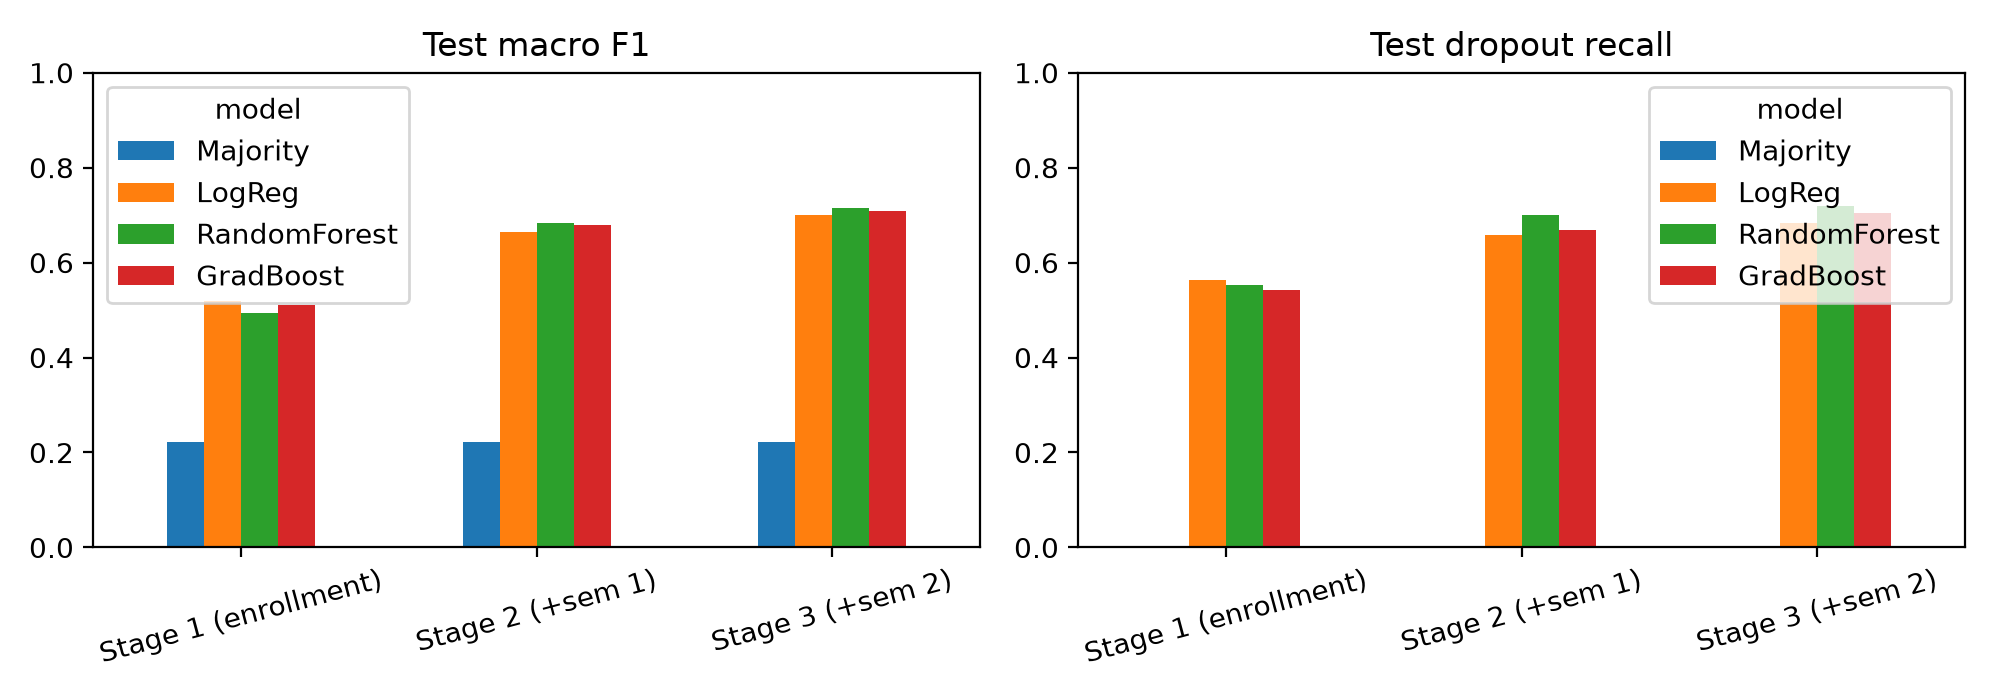
\includegraphics[width=0.8\textwidth]{stage_comparison.png}
  \caption{Test macro F1 and dropout recall by stage and model.}
  \label{fig:stages}
\end{figure*}

\begin{figure*}[t]
  \centering
  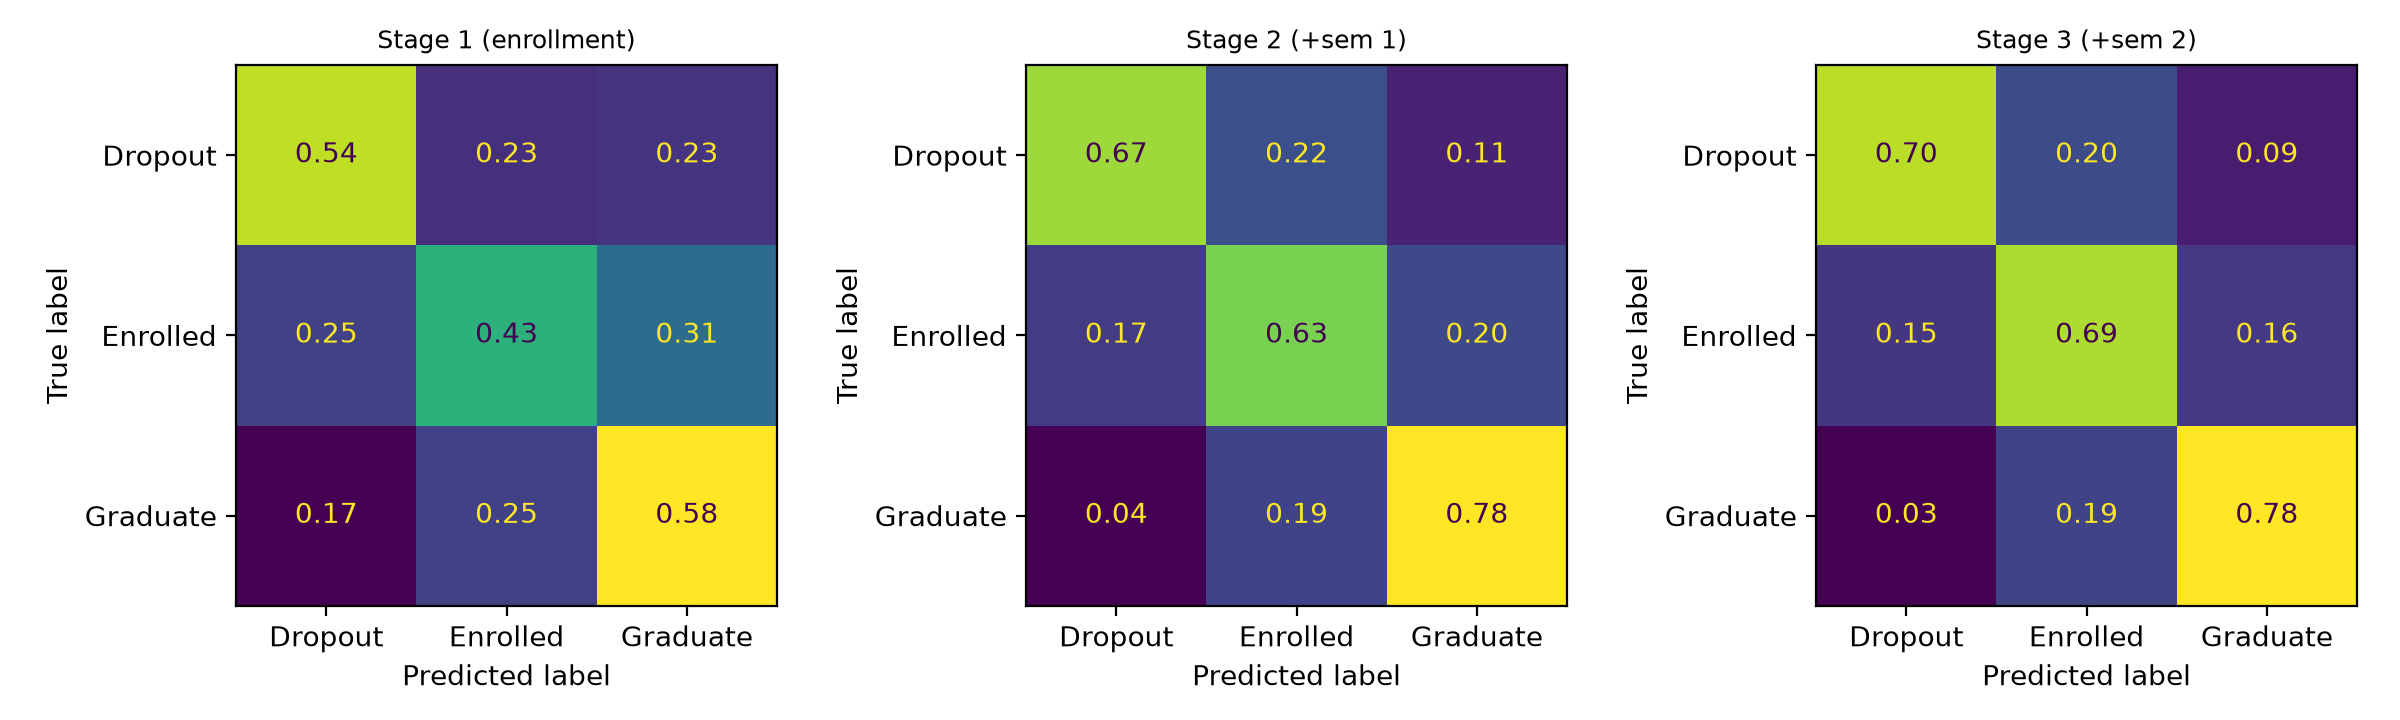
\includegraphics[width=0.85\textwidth]{confusion_gradboost.png}
  \caption{Row-normalized test confusion matrices for gradient boosting at each stage.}
  \label{fig:cm}
\end{figure*}

%% ---------------------------------------------------------------- 7
\section{Feedback and Plans}
\paragraph{TA feedback} We shared our draft report and results with our TA, Abdelaziz Serour, who confirmed that our evaluation setup (a single stratified split with cross-validation for tuning) and our baselines (the majority-class predictor and logistic regression) are sufficient for this milestone. He recommended that we prioritize: (1)~an error analysis of why Enrolled is difficult, using the confusion matrices to see which classes it is most often confused with; (2)~threshold tuning, which is worthwhile if identifying students at risk of dropping out is the priority, but since higher recall may reduce precision we should report both; (3)~explaining why Stage~2 provides most of the improvement, by identifying which of the new first-semester features are responsible; and (4)~using SHAP or permutation importance to find the features that contribute most at each stage. He also pointed out that Enrolled may represent students whose final outcome is not yet known, which could explain why it is hard to predict, and advised us to discuss this as a limitation rather than assuming that all errors come from model performance. Earlier, at the proposal stage, he advised keeping the three-class task and keeping Nationality out of the main setting.

\paragraph{Reflection} Our results show that Stage~1 is weak (macro F1 about 0.5), that the learned models are nearly tied, and that Enrolled is the main source of error. A first look at the confusion matrices in Figure~\ref{fig:cm} supports the TA's point about Enrolled: at Stage~1, 31\% of Enrolled students are predicted as Graduate and 25\% as Dropout, and even at Stage~3 they are split between the other two classes (15\% as Dropout, 16\% as Graduate). Because Enrolled students have not yet reached a final outcome, some of these errors may reflect genuine ambiguity in the label rather than a failure of the model, so Enrolled recall should be read with that limitation in mind. Because the models are so close, we also cannot yet claim that boosting is better than a regularized linear model, and our single split on 885 test students gives noisy comparisons.

\paragraph{Plans} Following the TA's recommendations: (1)~Carry out the Enrolled error analysis in more depth, examining which features and which students are involved in the Enrolled/Graduate and Enrolled/Dropout confusions. (2)~Tune decision thresholds on predicted probabilities to improve dropout recall and report precision alongside recall, so the trade-off is explicit. (3)~Compute permutation importance (and SHAP if time allows) for the best model at each stage, and use it to explain why Stage~2 provides most of the gain. (4)~Reduce noise in comparisons by repeating cross-validation with several seeds and reporting confidence intervals. (5)~Compare class weighting against SMOTE \citep{chawla2002}, add engineered features such as approval ratios and semester-to-semester changes, and ablate the macroeconomic features. (6)~Check the calibration of predicted probabilities and calibrate if needed. (7)~Run fairness checks (for example by gender and scholarship status, using group-wise recall) and test whether International status, Displaced or parental variables act as proxies for nationality; if time permits, run the secondary experiment including Nationality.
%% ---------------------------------------------------------------- Team
\section*{Team Contributions}

We both worked on and finished the code together. We both checked the final results table against the pipeline output.
\textbf{Anam Khan} wrote the Dataset, Features, Results and Evaluation, and Feedback and Plans sections. 
\textbf{Haniya Kashif} wrote the Introduction, Related Work and Implementation sections, reviewed the code and comments, and compiled the team contributions. 

\begin{thebibliography}{99}
 
  \bibitem[{Breiman(2001)}]{breiman2001}
  Leo Breiman. 2001.
  \newblock Random forests.
  \newblock \emph{Machine Learning}, 45(1):5--32.
   
  \bibitem[{Chawla et~al.(2002)Chawla, Bowyer, Hall, and Kegelmeyer}]{chawla2002}
  Nitesh~V. Chawla, Kevin~W. Bowyer, Lawrence~O. Hall, and W.~Philip Kegelmeyer. 2002.
  \newblock SMOTE: Synthetic minority over-sampling technique.
  \newblock \emph{Journal of Artificial Intelligence Research}, 16:321--357.
   
  \bibitem[{Chen and Guestrin(2016)}]{chen2016xgboost}
  Tianqi Chen and Carlos Guestrin. 2016.
  \newblock XGBoost: A scalable tree boosting system.
  \newblock In \emph{Proceedings of the 22nd ACM SIGKDD International Conference on Knowledge Discovery and Data Mining}, pages 785--794.
   
  \bibitem[{Friedman(2001)}]{friedman2001}
  Jerome~H. Friedman. 2001.
  \newblock Greedy function approximation: A gradient boosting machine.
  \newblock \emph{The Annals of Statistics}, 29(5):1189--1232.
   
  \bibitem[{Grinsztajn et~al.(2022)Grinsztajn, Oyallon, and Varoquaux}]{grinsztajn2022}
  L\'eo Grinsztajn, Edouard Oyallon, and Ga\"el Varoquaux. 2022.
  \newblock Why do tree-based models still outperform deep learning on typical tabular data?
  \newblock In \emph{Advances in Neural Information Processing Systems (Datasets and Benchmarks Track)}, volume~35.
   
  \bibitem[{Hardt et~al.(2016)Hardt, Price, and Srebro}]{hardt2016}
  Moritz Hardt, Eric Price, and Nathan Srebro. 2016.
  \newblock Equality of opportunity in supervised learning.
  \newblock In \emph{Advances in Neural Information Processing Systems}, volume~29, pages 3315--3323.
   
  \bibitem[{Ke et~al.(2017)Ke, Meng, Finley, Wang, Chen, Ma, Ye, and Liu}]{ke2017lightgbm}
  Guolin Ke, Qi~Meng, Thomas Finley, Taifeng Wang, Wei Chen, Weidong Ma, Qiwei Ye, and Tie-Yan Liu. 2017.
  \newblock LightGBM: A highly efficient gradient boosting decision tree.
  \newblock In \emph{Advances in Neural Information Processing Systems}, volume~30, pages 3146--3154.
   
  \bibitem[{Lundberg and Lee(2017)}]{lundberg2017}
  Scott~M. Lundberg and Su-In Lee. 2017.
  \newblock A unified approach to interpreting model predictions.
  \newblock In \emph{Advances in Neural Information Processing Systems}, volume~30, pages 4765--4774.
   
  \bibitem[{Martins et~al.(2021)Martins, Tolledo, Machado, Baptista, and Realinho}]{martins2021}
  M\'onica~V. Martins, Daniel Tolledo, Jorge Machado, Lu\'{\i}s M.~T. Baptista, and Valentim Realinho. 2021.
  \newblock Early prediction of student's performance in higher education: A case study.
  \newblock In \emph{Trends and Applications in Information Systems and Technologies (WorldCIST 2021), Volume 1}, Advances in Intelligent Systems and Computing, pages 166--175. Springer.
  \newblock DOI: 10.1007/\allowbreak 978-3-030-72657-7\_16.
   
  \bibitem[{Martins et~al.(2023)Martins, Baptista, Machado, and Realinho}]{martins2023}
  M\'onica~V. Martins, Lu\'{\i}s Baptista, Jorge Machado, and Valentim Realinho. 2023.
  \newblock Multi-class phased prediction of academic performance and dropout in higher education.
  \newblock \emph{Applied Sciences}, 13(8):4702.
   
  \bibitem[{Niculescu-Mizil and Caruana(2005)}]{niculescu2005}
  Alexandru Niculescu-Mizil and Rich Caruana. 2005.
  \newblock Predicting good probabilities with supervised learning.
  \newblock In \emph{Proceedings of the 22nd International Conference on Machine Learning}, pages 625--632.
   
  \bibitem[{Realinho et~al.(2022)Realinho, Machado, Baptista, and Martins}]{realinho2022}
  Valentim Realinho, Jorge Machado, Lu\'{\i}s Baptista, and M\'onica~V. Martins. 2022.
  \newblock Predicting student dropout and academic success.
  \newblock \emph{Data}, 7(11):146.
   
  \bibitem[{Tinto(1975)}]{tinto1975}
  Vincent Tinto. 1975.
  \newblock Dropout from higher education: A theoretical synthesis of recent research.
  \newblock \emph{Review of Educational Research}, 45(1):89--125.
   
  \end{thebibliography}
  
\end{document}